\section{Encriptado y desencriptado de un archivo wav}

\subsection{Organización de la cabecera}

Los datos de un archivo wav se encuentran administrados como header y los dados de audio como se muestra en la tabla \ref{table:wav_format}.

\begin{table}[H]
    \centering
    \begin{tabular}{ccl}
        \hline
        \textbf{Sección}      & \textbf{\begin{tabular}[c]{@{}l@{}}Tamaño\\ (bytes)\end{tabular}} & \textbf{Descripción}                   \\ \hline
        \multirow{2}{*}{RIFF} & 4                                  & Contiene las letras R, I, F y F        \\
                              & 4                                  & \begin{tabular}[c]{@{}l@{}}Entero positivo que almacena\\ el tamaño de los bytes restantes\end{tabular}              \\ \hline
                              & 4                                  & Contienen las letras: W, A, V y E.     \\
                              & 4                                  & Contiene los caracteres F, M, T        \\
                              & 4                                  & \begin{tabular}[c]{@{}l@{}}Entero positivo que indica el tamaño\\ en bytes del resto del bloque\end{tabular}              \\
        WAVE                  & 2                                  & \begin{tabular}[c]{@{}l@{}}Entero positivo de 16 bits que indica \\ el tipo de grabación. Un 1 significa PCM.\end{tabular}              \\
                              & 2                                  & Número de canales                      \\
                              & 4                                  & Frecuencia de muestreo expresada en Hz \\
                              & 4                                  & Número promedio de bytes por segundo   \\
                              & 2                                  & \begin{tabular}[c]{@{}l@{}}Número de bytes usados en el archivo para\\ cada muestra\end{tabular}              \\
                              & 2                                  & Bits por muestra                       \\ \hline
                              & 4                                  & Contiene las letras d, a, t, a         \\
        data                  & 4                                  & \begin{tabular}[c]{@{}l@{}}Entero positivo que indica el espacio\\ de bytes que ocupan los datos\end{tabular}              \\
                              & n                                  & Datos                                  \\ \hline
    \end{tabular}
    \caption{Organización de los datos en un archivo de formato wav.}
    \label{table:wav_format}
\end{table}

Esta organización hace que los primeros 44 bytes no sean modificados, ya que es información del archivo y no sus datos. Al ser los archivos de muestra de un audio mono, entonces estos tiene un tamaño de 16 bits por muestra, esto se puede ver en las figuras \ref{fig:ftea_information} y \ref{fig:mtea_information}.

\begin{minipage}{8.2cm}
    \begin{figure}[H]
        \centering
        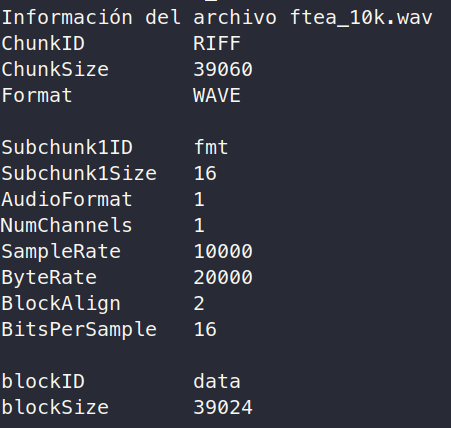
\includegraphics[width=7.5cm]{Graphics/ftea_10k_information.png}
        \caption{Información del archivo \file{ftea\_10k.wav}}
        \label{fig:ftea_information}
    \end{figure}
\end{minipage}
\hspace{0.5cm}
\begin{minipage}{8.2cm}
    \begin{figure}[H]
        \centering
        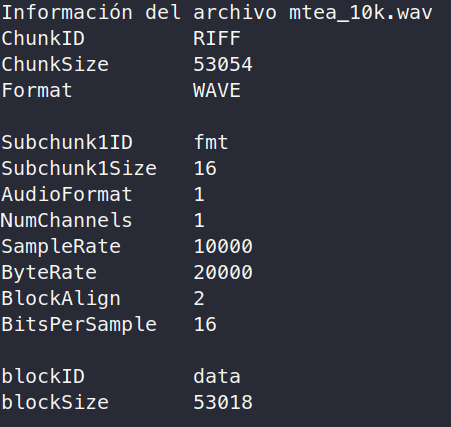
\includegraphics[width=7.5cm]{Graphics/mtea_10k_information.png}
        \caption{Información del archivo \file{mtea\_10k.wav}}
        \label{fig:mtea_information}
    \end{figure}
\end{minipage}

Si estos fueran un audio stereo, entocnes el número de bits por muestra seria 32, 16 para el audio izquiero y 16 para el derecho. Es por ello que se implemento un arreglo de dimension dinámica para guardar cada muestra del archivo.

\subsection{Lectura y organización de los datos}

La lectura de los datos de la cabecera serán guardados en tipos definidos. Estos tipos se encuentran en el archivo \file{wave.h}. Este proceso no es propio, se encontro un repositorio en GitHub, el cual realiza modificaciones al sonido y se implemento el uso de sus lecturas de los datos. Estos reposiorotios son los siguientes: \href{https://github.com/fabrizzio-gz/wav/}{Lectura de los datos}, \href{https://topic.alibabacloud.com/a/c-language-parsing-wav-audio-files_1_31_30000716.html}{Estructura de los tipos}.

El arreglo de datos es de tipo short para que estos coincidan con los 16 bits que tiene cada muestra de audio. Al tener las muestras de audio organizadas en arreglos es más sencillo realizar el paso por cada uno de estos datos.

\subsection{Encriptación y desencriptación}

\subsubsection{Mapa caótico}

En la teoría del caos se describen comportamientos de sistemas dinámicos los cuales se ven afectados por sus condiciones iniciales\cite{ott_2002}. En este caso tendremos unas condiciones iniciales llamadas $X_{i,0}$, donde i, es el número de llaves. Al tener 2 bytes por muestra, dividiremos esto en datos de 1 byte. Entonces el número de llaves serán 2.

El mapa caótico que se uso esta definido en la ecuación \ref{eq:chaotic_map}.

\begin{equation}
    X_{i,j} = b X_{i,j-1} + \left \lfloor \frac{X_{i,j-1}}{2^m} \right \rfloor + \epsilon \& \bigotimes_{k=1}^3 X_{k,j-1} \label{eq:chaotic_map}
\end{equation}

donde $\epsilon, b, m \in \mathbb{N}$ y $3<m<8$.

\subsubsection{Algoritmo}

El algoritmo creado para aplicar el mapa caótico de la ecuación \ref{eq:chaotic_map} es el siguiente:

\begin{algorithm}[H]
    \caption{Encriptado y desencriptado}
    \KwInput{$data,keys$}
    \KwOutput{$data$}
    map $\gets$ keys\\
    \For{$i=1,$n\_samples}
    {
        bytes $\gets$ data[i]\\
        \For{j=1,2}
        {
            bytes[j] $\gets$ bytes[j]$\bigotimes$map[j]\\
            map[j] $\gets f(map[j],m,\epsilon$,b)\\
        }
    }
\end{algorithm}